\documentclass[11pt]{article}
\usepackage[margin=0.9in]{geometry}
\usepackage{amsmath,amssymb,amsthm}
\usepackage{tikz}
\usepackage{pgfplots}
\pgfplotsset{compat=1.18}
\usetikzlibrary{arrows.meta,positioning,calc}
\usepackage{xcolor}
\definecolor{ink}{HTML}{1A2238}
\definecolor{acc}{HTML}{7C3AED}
\definecolor{acc2}{HTML}{0EA5A4}
\definecolor{warm}{HTML}{D97706}
\usepackage{titlesec}\titleformat{\section}{\large\bfseries\color{ink}}{\thesection}{0.6em}{}
\newtheorem{lemma}{Lemma}\newtheorem{theorem}{Theorem}
\usepackage{parskip}
\title{\bfseries\color{ink} Stepping Through the Door\\[2pt]\large A Tao-style almost-all theorem for the renewal map, and how close we are}
\author{BB(6) research program}\date{2026-09-07}
\begin{document}\maketitle

\noindent\textbf{One-line status.} The obstruction feared by the transfer-operator scaffold---parabolic intermittency---\emph{does not exist}: a parity theorem shows the neutral generator $T$ is never iterated. This reduces the almost-all-seeds theorem from ``one hard lemma'' to ``two checkable Rychlik constants,'' both strongly supported numerically. Not yet a finished proof; materially closer to the door.

\section{The target, and Tao's parallel}
Tao (2019) \emph{proved} that almost every Collatz orbit attains almost bounded values, via a stationary measure for the Syracuse map---while leaving every specific $n$ Collatz-hard. Our renewal map $R$ (governing the dossier-2/3 orbit) poses the exact analogue: \emph{do almost all seeds avoid the fatal set?} The machinery is a transfer operator rather than Syracuse random variables, but the shape---almost-all reachable, specific orbit Collatz-hard---is identical.

\smallskip\noindent The map, on $(a,b)$, with $\beta(a)=a-1$ ($a$ odd) or $a-2$ ($a$ even):
\[ T:\ b\ \text{even}\ \mapsto (a{+}6,\,b{-}3);\quad C:\ b<\beta \mapsto(\ldots);\quad F:\ b>\beta \mapsto(3a{+}6,\,b{-}\beta{-}4). \]
Linear parts: $T=\bigl[\begin{smallmatrix}1&0\\0&1\end{smallmatrix}\bigr]$ (parabolic), $C=\bigl[\begin{smallmatrix}0&3\\1&-1\end{smallmatrix}\bigr]$, $F=\bigl[\begin{smallmatrix}3&0\\-1&1\end{smallmatrix}\bigr]$ (det $\pm3$, the Collatz multiplier).

\section{The obstruction that isn't: no intermittency}
\begin{lemma}[Parity grammar, proven exhaustively]
$\beta(a)$ is always even. Hence $T$ outputs $b{-}3$ (odd), $C$ outputs an even $b'$, $F$ outputs an odd $b'$. The symbol grammar is
\[ T\to\{C,F\},\qquad C\to T,\qquad F\to\{C,F\}, \]
and \textbf{$TT$ is impossible}: the neutral generator $T$ is never iterated---it occurs only inside an isolated $C\!\to\!T$ pair.
\end{lemma}
There is thus no neutral orbit segment of length $>1$, so \emph{no Pomeau--Manneville intermittency}. The cusp is touched but never followed. This is the fact that unlocks everything below.

\begin{center}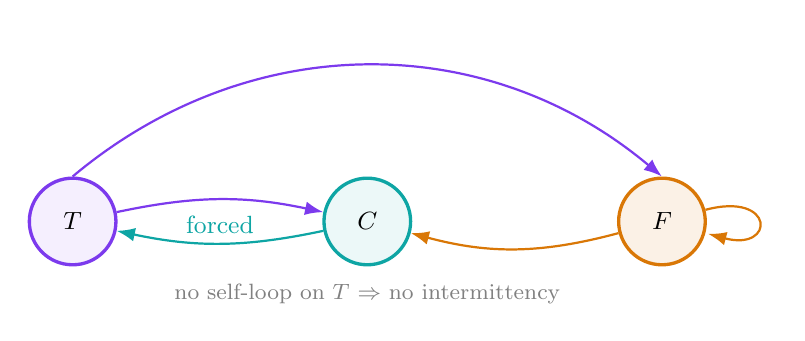
\begin{tikzpicture}[>=Latex,node distance=26mm,every node/.style={font=\small}]
\node[circle,draw=acc,very thick,fill=acc!8,minimum size=11mm](T){$T$};
\node[circle,draw=acc2,very thick,fill=acc2!8,minimum size=11mm,right=of T](C){$C$};
\node[circle,draw=warm,very thick,fill=warm!10,minimum size=11mm,right=of C](F){$F$};
\draw[->,acc2,thick] (C) to[bend left=12] node[above]{forced} (T);
\draw[->,acc,thick] (T) to[bend left=12] (C);
\draw[->,acc,thick] (T.north) to[bend left=40] (F.north);
\draw[->,warm,thick] (F) to[bend left=15] (C);
\draw[->,warm,thick] (F) edge[loop right] ();
\node[below=1mm of C,gray,font=\footnotesize]{no self-loop on $T$ $\Rightarrow$ no intermittency};
\end{tikzpicture}\end{center}

\section{The induced map is uniformly expanding}
Inducing on the $F$-section in the scale-invariant coordinate $z=o/(o{+}\beta)$, $o=b{-}\beta$:

\begin{center}
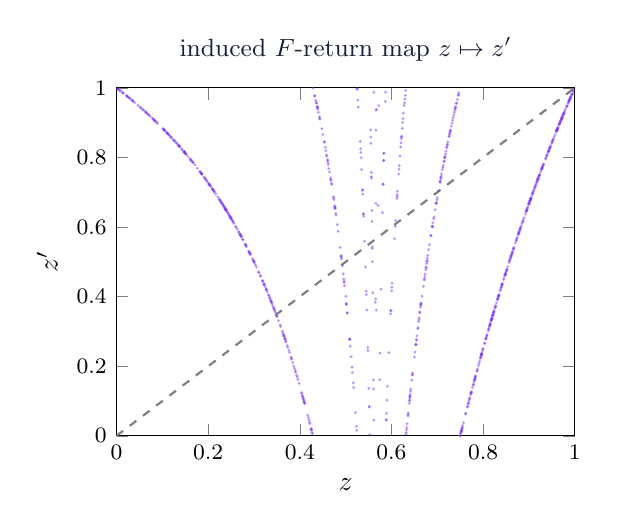
\begin{tikzpicture}
\begin{axis}[width=7.4cm,height=6cm,title={\small induced $F$-return map $z\mapsto z'$},xlabel={$z$},ylabel={$z'$},xmin=0,xmax=1,ymin=0,ymax=1,tick label style={font=\footnotesize},title style={color=ink}]
\addplot[only marks,mark=*,mark size=0.35pt,acc,opacity=0.35] coordinates{(0.8968,0.6547) (0.8566,0.4979) (0.5175,0.139) (0.132,0.8399) (0.6401,0.1089) (0.9608,0.8777) (0.2496,0.626) (0.7164,0.8001) (0.5035,0.3535) (0.4677,0.7365) (0.0236,0.9756) (0.5751,0.2376) (0.6067,0.5666) (0.3273,0.4193) (0.3886,0.1937) (0.4536,0.8448) (0.7113,0.7655) (0.6778,0.5032) (0.5582,0.5428) (0.8341,0.4033) (0.9112,0.7078) (0.0878,0.9006) (0.6735,0.4649) (0.2529,0.6185) (0.357,0.3187) (0.7738,0.123) (0.6247,0.901) (0.3382,0.3841) (0.5088,0.2774) (0.6158,0.7524) (0.8663,0.537) (0.1467,0.8176) (0.5867,0.961) (0.9785,0.934) (0.1108,0.87) (0.6721,0.4512) (0.6416,0.128) (0.5088,0.2779) (0.4363,0.9563) (0.5834,0.8121) (0.8507,0.4734) (0.727,0.8677) (0.4967,0.4416) (0.8602,0.5125) (0.3983,0.1508) (0.4902,0.5177) (0.8339,0.4024) (0.329,0.414) (0.2123,0.7039) (0.9709,0.91) (0.4069,0.1104) (0.6334,0.0236) (0.5463,0.3616) (0.9534,0.8532) (0.0216,0.9778) (0.1824,0.7589) (0.9386,0.8039) (0.818,0.3325) (0.943,0.8186) (0.989,0.9665) (0.0845,0.9047) (0.4092,0.0997) (0.535,0.7653) (0.2372,0.6531) (0.7969,0.2355) (0.3267,0.421) (0.9892,0.9672) (0.754,0.0211) (0.795,0.2266) (0.9177,0.7308) (0.2167,0.6952) (0.6863,0.5762) (0.3185,0.4463) (0.4221,0.0346) (0.9459,0.8284) (0.8063,0.2792) (0.7207,0.8281) (0.3658,0.2861) (0.6513,0.2408) (0.9528,0.8513) (0.6814,0.5348) (0.6127,0.6932) (0.5834,0.8121) (0.8347,0.4059) (0.2376,0.6522) (0.9661,0.8947) (0.9759,0.9259) (0.249,0.6272) (0.6235,0.8838) (0.5772,0.4215) (0.8575,0.5016) (0.973,0.9167) (0.5915,0.1426) (0.7306,0.8901) (0.8922,0.6375) (0.2018,0.724) (0.4286,0.9997) (0.9876,0.9622) (0.6404,0.1132) (0.1599,0.7968) (0.2538,0.6165) (0.7511,0.006) (0.41,0.0954) (0.8153,0.3202) (0.2713,0.5749) (0.4382,0.9451) (0.9043,0.6826) (0.2905,0.5259) (0.9036,0.6799) (0.4172,0.0597) (0.9939,0.9814) (0.3145,0.4585) (0.8259,0.3677) (0.1479,0.8157) (0.8407,0.4316) (0.3809,0.2261) (0.5016,0.3786) (0.972,0.9136) (0.0517,0.9445) (0.427,0.0087) (0.3322,0.4036) (0.7123,0.772) (0.7501,0.0004) (0.1481,0.8154) (0.9043,0.6823) (0.7965,0.2335) (0.233,0.662) (0.1509,0.811) (0.3618,0.3011) (0.8582,0.5044) (0.5586,0.5006) (0.3823,0.2203) (0.8673,0.5411) (0.004,0.996) (0.4383,0.9446) (0.894,0.6444) (0.9517,0.8478) (0.8064,0.2797) (0.6409,0.1188) (0.2021,0.7234) (0.5277,0.9447) (0.8778,0.5824) (0.2211,0.6864) (0.4734,0.6868) (0.0794,0.9112) (0.8322,0.3949) (0.9298,0.7736) (0.7814,0.161) (0.7474,0.9862) (0.4434,0.9129) (0.6329,0.0172) (0.6443,0.1602) (0.4199,0.0458) (0.74,0.9448) (0.6166,0.7664) (0.2507,0.6235) (0.4765,0.6585) (0.823,0.3547) (0.762,0.0628) (0.7746,0.1271) (0.8833,0.6037) (0.2923,0.5211) (0.7191,0.8176) (0.6461,0.1807) (0.105,0.8779) (0.322,0.4358) (0.2724,0.5723) (0.171,0.7785) (0.2485,0.6283) (0.8615,0.5176) (0.2286,0.6712) (0.0148,0.9849) (0.2384,0.6504) (0.6293,0.9682) (0.1428,0.8235) (0.4252,0.0187) (0.8513,0.4758) (0.2306,0.6671) (0.2565,0.6102) (0.4247,0.0207) (0.7419,0.9554) (0.8894,0.6268) (0.8851,0.6105) (0.4689,0.7262) (0.6285,0.9572) (0.9911,0.973) (0.6279,0.9494) (0.63,0.9786) (0.0573,0.9379) (0.022,0.9774) (0.6083,0.6023) (0.6556,0.2873) (0.9609,0.8779) (0.3643,0.2914) (0.4904,0.5164) (0.8187,0.3358) (0.9725,0.915) (0.3223,0.435) (0.8589,0.5073) (0.2758,0.5638) (0.5088,0.2778) (0.0398,0.958) (0.8138,0.3135) (0.4679,0.7342) (0.4762,0.6612) (0.0558,0.9397) (0.4623,0.7796) (0.9616,0.8804) (0.008,0.9919) (0.2995,0.5013) (0.7678,0.0928) (0.832,0.3943) (0.1382,0.8306) (0.9127,0.7129) (0.9364,0.7961) (0.467,0.7416) (0.6595,0.3285) (0.622,0.8594) (0.1935,0.7392) (0.0655,0.9282) (0.2755,0.5646) (0.2967,0.509) (0.1101,0.871) (0.6642,0.3757) (0.7556,0.0294) (0.7662,0.0845) (0.1819,0.7599) (0.7095,0.753) (0.4881,0.5411) (0.7524,0.0126) (0.3446,0.3624) (0.636,0.0574) (0.6187,0.8045) (0.1497,0.813) (0.6533,0.2619) (0.4965,0.4439) (0.8217,0.3491) (0.3029,0.4918) (0.9093,0.7007) (0.491,0.5087) (0.8668,0.539) (0.6893,0.6012) (0.8789,0.5867) (0.9915,0.9743) (0.6501,0.2268) (0.901,0.6705) (0.9296,0.7729) (0.9716,0.9124) (0.3846,0.2107) (0.9434,0.82) (0.6893,0.6012) (0.4975,0.4319) (0.07,0.9228) (0.2603,0.6014) (0.6124,0.6881) (0.4837,0.5881) (0.5167,0.1524) (0.7361,0.9225) (0.7168,0.8027) (0.3453,0.3601) (0.2272,0.6742) (0.0644,0.9296) (0.6319,0.0043) (0.1864,0.7519) (0.8448,0.4488) (0.8996,0.6651) (0.8521,0.4791) (0.9865,0.9589) (0.208,0.7122) (0.3222,0.4352) (0.2835,0.5442) (0.5101,0.2577) (0.6862,0.5751) (0.1196,0.8577) (0.214,0.7005) (0.9756,0.9249) (0.8777,0.5821) (0.0816,0.9084) (0.3107,0.4695) (0.583,0.7924) (0.6749,0.4778) (0.9684,0.9021) (0.9507,0.8443) (0.0349,0.9634) (0.3699,0.2702) (0.1513,0.8104) (0.0669,0.9266) (0.6534,0.2632) (0.5829,0.7905) (0.7,0.6843) (0.9196,0.7376) (0.9132,0.7148) (0.5592,0.4107) (0.1629,0.792) (0.8483,0.4635) (0.4079,0.1058) (0.9313,0.7788) (0.27,0.5782) (0.8189,0.3367) (0.7062,0.7299) (0.9829,0.9479) (0.6922,0.6242) (0.9466,0.8309) (0.1248,0.8503) (0.698,0.6693) (0.6014,0.4383) (0.3942,0.1689) (0.7219,0.8361) (0.7965,0.2336) (0.8538,0.4862) (0.6264,0.9273) (0.9077,0.6951) (0.3901,0.1869) (0.7464,0.9808) (0.2665,0.5866) (0.5392,0.6372) (0.5893,0.0646) (0.3268,0.421) (0.9727,0.9158) (0.4326,0.9778) (0.0826,0.9072) (0.6831,0.5495) (0.5817,0.7236) (0.8292,0.382) (0.8423,0.4383) (0.6756,0.4833) (0.3375,0.3863) (0.5392,0.638) (0.5706,0.6616) (0.7786,0.1468) (0.7925,0.2145) (0.195,0.7365) (0.3503,0.3429) (0.6209,0.842) (0.3633,0.2955) (0.7528,0.0147) (0.8174,0.3298) (0.6254,0.9119) (0.8189,0.3366) (0.0075,0.9924) (0.5215,0.0668) (0.1133,0.8666) (0.1555,0.8038) (0.7179,0.8097) (0.8647,0.5305) (0.8596,0.5102) (0.0267,0.9723) (0.2129,0.7028) (0.6606,0.3393) (0.8235,0.357) (0.4947,0.4656) (0.7232,0.8443) (0.4769,0.6542) (0.4428,0.9167) (0.5337,0.7992) (0.1038,0.8795) (0.8867,0.6165) (0.0703,0.9225) (0.3431,0.3674) (0.5236,0.0275) (0.5507,0.1366) (0.6132,0.703) (0.8124,0.3072) (0.8479,0.4617) (0.698,0.6693) (0.9182,0.7326) (0.5552,0.8412) (0.4558,0.8291) (0.322,0.4358) (0.9198,0.7383) (0.0632,0.931) (0.3319,0.4046) (0.5904,0.1024) (0.9879,0.9633) (0.9623,0.8823) (0.7659,0.0829) (0.969,0.9041) (0.7866,0.186) (0.2829,0.5457) (0.8112,0.3018) (0.3344,0.3966) (0.7163,0.7994) (0.1425,0.824) (0.406,0.1147) (0.2009,0.7256) (0.5414,0.5593) (0.827,0.3722) (0.4767,0.6561) (0.8864,0.6154) (0.8976,0.6578) (0.4928,0.4889) (0.8961,0.6521) (0.8181,0.3329) (0.1096,0.8717) (0.5888,0.0459) (0.795,0.2263) (0.3673,0.2803) (0.5664,0.8788) (0.6342,0.035) (0.4046,0.1217) (0.9229,0.7493) (0.9608,0.8776) (0.8639,0.5272) (0.721,0.8301) (0.435,0.9637) (0.8264,0.3697) (0.7077,0.7401) (0.298,0.5054) (0.6636,0.3701) (0.3362,0.3905) (0.9254,0.7581) (0.4255,0.0166) (0.3776,0.2396) (0.9618,0.881) (0.1616,0.794) (0.9086,0.6982) (0.8459,0.4534) (0.9851,0.9547) (0.7147,0.7883) (0.66,0.3335) (0.1927,0.7409) (0.7439,0.9667) (0.7321,0.8988) (0.9944,0.983) (0.6668,0.4015) (0.3368,0.3886) (0.7528,0.0149) (0.0287,0.9701) (0.8786,0.5855) (0.6456,0.1748) (0.2912,0.524) (0.4212,0.0392) (0.5036,0.3526) (0.6795,0.5187) (0.9169,0.7283) (0.3817,0.2228) (0.9739,0.9195) (0.1265,0.8478) (0.3344,0.3965) (0.8185,0.335) (0.4607,0.792) (0.7532,0.017) (0.9753,0.924) (0.6366,0.0651) (0.2398,0.6475) (0.771,0.1089) (0.9601,0.8754) (0.0118,0.988) (0.8142,0.3152) (0.537,0.7063) (0.9765,0.9278) (0.1054,0.8773) (0.2814,0.5497) (0.9616,0.8801) (0.9674,0.8988) (0.7738,0.1229) (0.8231,0.3551) (0.8154,0.3209) (0.3193,0.444) (0.1514,0.8103) (0.9231,0.7502) (0.1242,0.8511) (0.5562,0.757) (0.4361,0.9576) (0.3008,0.4977) (0.7571,0.0373) (0.8632,0.5248) (0.9313,0.7787) (0.3245,0.428) (0.821,0.3458) (0.3383,0.3838) (0.4743,0.6788) (0.8663,0.5372) (0.5434,0.4857) (0.2433,0.6399) (0.2894,0.5287) (0.4252,0.0179) (0.2095,0.7093) (0.1973,0.7323) (0.9401,0.8088) (0.0345,0.9638) (0.5576,0.6166) (0.184,0.7562) (0.393,0.1744) (0.9869,0.9601) (0.5374,0.6948) (0.6992,0.6782) (0.7623,0.0644) (0.2104,0.7076) (0.4818,0.6071) (0.4481,0.8827) (0.3737,0.2552) (0.6394,0.1007) (0.387,0.2004) (0.5529,0.0034) (0.8518,0.4782) (0.5743,0.161) (0.4061,0.1142) (0.103,0.8806) (0.914,0.7178) (0.2466,0.6327) (0.0604,0.9344) (0.5679,0.938) (0.4392,0.9392) (0.9025,0.6759) (0.9427,0.8178) (0.0521,0.9441) (0.047,0.9499) (0.9201,0.7395) (0.5618,0.9873) (0.6717,0.448) (0.8808,0.5941) (0.5487,0.2447) (0.5517,0.0828) (0.8951,0.6484) (0.0853,0.9038) (0.391,0.1832) (0.2546,0.6146) (0.7547,0.0247) (0.27,0.5781) (0.4616,0.785) (0.5664,0.9364) (0.9198,0.7384) (0.6576,0.3083) (0.7284,0.8768) (0.9275,0.7654) (0.5817,0.7231) (0.6728,0.4581) (0.2376,0.6522) (0.7257,0.8599) (0.6122,0.6826) (0.9941,0.9822) (0.1672,0.7848) (0.191,0.7438) (0.7802,0.1547) (0.037,0.961) (0.4407,0.93) (0.7958,0.2301) (0.5516,0.085) (0.9024,0.6755) (0.1649,0.7887) (0.2096,0.7091) (0.819,0.3368) (0.2278,0.6729) (0.7827,0.167) (0.7817,0.1623) (0.881,0.595) (0.1357,0.8343) (0.662,0.3541) (0.7788,0.1477) (0.6978,0.6678) (0.5803,0.6416) (0.231,0.6661) (0.8484,0.4638) (0.2919,0.5222) (0.6776,0.5015) (0.8393,0.4257) (0.4385,0.9431) (0.1195,0.8578) (0.2816,0.5491) (0.9607,0.8774) (0.8203,0.3426) (0.2338,0.6603) (0.9371,0.7986) (0.537,0.7067) (0.5563,0.7411) (0.742,0.9561) (0.7375,0.9304) (0.2395,0.6481) (0.9453,0.8265) (0.7261,0.8623) (0.2707,0.5763) (0.8148,0.318) (0.1307,0.8417) (0.5657,0.3937) (0.3582,0.3142) (0.5582,0.5386) (0.0041,0.9959) (0.8036,0.2667) (0.8798,0.59) (0.9597,0.874) (0.7677,0.092) (0.2457,0.6345) (0.7879,0.1922) (0.2672,0.585) (0.1855,0.7535) (0.1154,0.8636) (0.9227,0.7485) (0.2257,0.6772) (0.7964,0.2331) (0.7871,0.1885) (0.9473,0.8332) (0.5651,0.3839) (0.9824,0.9464) (0.4505,0.8661) (0.9191,0.7359) (0.4606,0.7927) (0.1014,0.8828) (0.6532,0.2618) (0.8489,0.4662) (0.2608,0.6001) (0.9702,0.9077) (0.8998,0.6659) (0.3694,0.272) (0.4328,0.9764) (0.1182,0.8597) (0.9495,0.8403) (0.8033,0.2655) (0.4587,0.8073) (0.2244,0.6797) (0.6221,0.861) (0.1474,0.8165) (0.8242,0.3599) (0.9283,0.7683) (0.7081,0.743) (0.5945,0.2387) (0.6388,0.093) (0.4104,0.0935) (0.4738,0.6836) (0.5121,0.2274) (0.3434,0.3666) (0.2486,0.6282) (0.6644,0.3781) (0.6457,0.1761) (0.5451,0.4162) (0.2301,0.6681) (0.9288,0.7702) (0.9039,0.6812) (0.8335,0.4007) (0.7274,0.8702) (0.9044,0.6828) (0.136,0.8339) (0.4785,0.6391) (0.9802,0.9394) (0.8477,0.4611) (0.9447,0.8243) (0.5986,0.3603) (0.9015,0.6723) (0.9827,0.9473) (0.7812,0.16) (0.8229,0.3542) (0.4438,0.9105) (0.9393,0.8061) (0.5873,0.9878) (0.9321,0.7814) (0.8319,0.3934) (0.7501,0.0005) (0.1852,0.7541) (0.496,0.4507) (0.7222,0.8378) (0.409,0.1004) (0.2473,0.631) (0.1859,0.7528) (0.3102,0.471) (0.9001,0.6671) (0.6955,0.65) (0.408,0.1054) (0.2811,0.5504) (0.9208,0.7419) (0.7518,0.0096) (0.9275,0.7655) (0.7386,0.9369) (0.514,0.1974) (0.9419,0.8149) (0.2434,0.6397) (0.9882,0.9642) (0.975,0.9232) (0.7739,0.1236) (0.8213,0.3472) (0.5982,0.3512) (0.8723,0.5609) (0.2691,0.5802) (0.5486,0.2542) (0.1765,0.7692) (0.2357,0.6564) (0.8737,0.5662) (0.1861,0.7526) (0.9552,0.8594) (0.5332,0.8142) (0.1629,0.7918) (0.0034,0.9966) (0.1666,0.7858) (0.9433,0.8195) (0.2634,0.594) (0.5724,0.949) (0.8082,0.2879) (0.2029,0.7219) (0.404,0.1244) (0.7289,0.8797) (0.85,0.4707) (0.6363,0.0612) (0.9899,0.9695) (0.6422,0.1344) (0.479,0.6347) (0.7833,0.1698) (0.561,0.1348) (0.8412,0.4338) (0.8373,0.4169) (0.4536,0.8444) (0.9229,0.7493) (0.465,0.7586) (0.5242,0.0156) (0.2035,0.7208) (0.8342,0.4039) (0.5251,0.9984) (0.9103,0.7045) (0.3192,0.4444) (0.0023,0.9977) (0.6545,0.2751) (0.5252,0.996) (0.03,0.9688) (0.6769,0.4956) (0.8614,0.5175) (0.3415,0.3729) (0.5547,0.8793) (0.8397,0.4274) (0.7461,0.9789) (0.6091,0.6186) (0.3656,0.2868) (0.7027,0.704) (0.8632,0.5248) (0.8333,0.4) (0.4693,0.7224) (0.5563,0.7449) (0.555,0.8585) (0.6786,0.5104) (0.8313,0.3912) (0.882,0.5986) (0.2886,0.531) (0.4906,0.5136) (0.967,0.8978) (0.7335,0.9071) (0.6907,0.6125) (0.9286,0.7692) (0.477,0.6539) (0.9082,0.6968) (0.7068,0.7342) (0.4637,0.7684) (0.365,0.2891) (0.2398,0.6475) (0.2996,0.501) (0.9913,0.9736) (0.5328,0.8252) (0.29,0.5273) (0.6006,0.4168) (0.7839,0.1727) (0.797,0.236) (0.9218,0.7457) (0.9571,0.8654) (0.2049,0.7181) (0.9974,0.9922) (0.4571,0.8194) (0.7706,0.1068) (0.631,0.9925) (0.9148,0.7207) (0.6323,0.0093) (0.3135,0.4612) (0.8811,0.5951) (0.821,0.3457) (0.8416,0.4353) (0.5668,0.3612) (0.6405,0.1139) (0.1478,0.8159) (0.2995,0.5014) (0.9006,0.6691) (0.6217,0.8545) (0.7899,0.2019) (0.0733,0.9188) (0.7975,0.2383) (0.2723,0.5725) (0.9628,0.8842) (0.6202,0.8302) (0.2371,0.6532) (0.7998,0.2491) (0.9713,0.9113) (0.5888,0.0458) (0.7521,0.0111) (0.9933,0.9797) (0.713,0.7773) (0.6895,0.6023) (0.4186,0.0528) (0.4274,0.0063) (0.9064,0.6901) (0.1278,0.8459) (0.1145,0.8648) (0.2362,0.6553) (0.777,0.1391) (0.3468,0.3547) (0.2248,0.679) (0.754,0.0212) (0.951,0.8455) (0.438,0.9462) (0.2109,0.7066) (0.1377,0.8314) (0.8413,0.4342) (0.5608,0.1609) (0.7348,0.9149) (0.9659,0.8941) (0.8212,0.3468) (0.7149,0.79) (0.9157,0.7239) (0.9631,0.8851) (0.9694,0.9052) (0.8621,0.52) (0.9456,0.8273) (0.8274,0.3741) (0.1109,0.8699) (0.8727,0.5626) (0.7282,0.875) (0.7061,0.7288) (0.1049,0.8781) (0.3958,0.1621) (0.8765,0.5771) (0.5017,0.3775) (0.9041,0.6819) (0.7818,0.1629) (0.783,0.1686) (0.6757,0.485) (0.1487,0.8145) (0.8382,0.4209) (0.3535,0.3312) (0.0895,0.8983) (0.9635,0.8863) (0.5662,0.668) (0.6648,0.382) (0.601,0.4268) (0.3397,0.3789) (0.1479,0.8158) (0.8746,0.5698) (0.9674,0.8989) (0.6171,0.7764) (0.5573,0.6479) (0.895,0.6481) (0.9981,0.9944) (0.0345,0.9638) (0.8773,0.5805) (0.7085,0.7459) (0.3678,0.2782) (0.0783,0.9126) (0.8122,0.3062) (0.7987,0.2441) (0.376,0.2459) (0.1354,0.8348) (0.8076,0.2855) (0.5453,0.4062) (0.9771,0.9297) (0.9967,0.99) (0.6928,0.6288) (0.5149,0.1822) (0.6622,0.3561) (0.025,0.9741) (0.6645,0.3789) (0.0831,0.9065) (0.8159,0.3232) (0.5267,0.9649) (0.3499,0.3442) (0.7911,0.2079) (0.2382,0.651) (0.4592,0.8036) (0.5394,0.631) (0.7729,0.1183) (0.2332,0.6616) (0.0143,0.9854) (0.903,0.6777) (0.7399,0.9443) (0.3052,0.4854) (0.8706,0.5543) (0.8878,0.6208) (0.8,0.2501) (0.6698,0.4296) (0.2509,0.6229) (0.7698,0.1031) (0.6396,0.1031) (0.4104,0.0937) (0.8953,0.649) (0.5015,0.3809) (0.6579,0.3111) (0.7688,0.0978) (0.861,0.5155) (0.8942,0.645) (0.2042,0.7194) (0.3679,0.278) (0.1973,0.7322) (0.1022,0.8816) (0.1362,0.8336) (0.3726,0.2595) (0.2412,0.6444) (0.5615,0.045) (0.5319,0.8465) (0.6546,0.2764) (0.9023,0.6752) (0.9905,0.9713) (0.9713,0.9113) (0.8088,0.2907) (0.5985,0.3596) (0.7941,0.2222) (0.8487,0.465) (0.5006,0.4015) (0.7392,0.9406) (0.8062,0.2789)};
\addplot[gray,dashed,thick] coordinates{(0,0)(1,1)};
\end{axis}\end{tikzpicture}\hfill
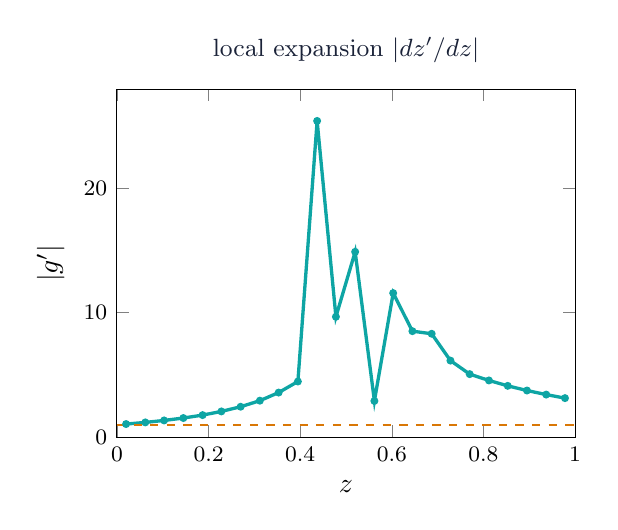
\begin{tikzpicture}
\begin{axis}[width=7.4cm,height=6cm,title={\small local expansion $|dz'/dz|$},xlabel={$z$},ylabel={$|g'|$},xmin=0,xmax=1,ymin=0,tick label style={font=\footnotesize},title style={color=ink}]
\addplot[acc2,very thick,mark=*,mark size=0.8pt] coordinates{(0.02,1.056) (0.062,1.188) (0.103,1.346) (0.145,1.539) (0.187,1.774) (0.228,2.069) (0.27,2.445) (0.312,2.931) (0.353,3.582) (0.395,4.469) (0.437,25.369) (0.478,9.66) (0.52,14.871) (0.562,2.911) (0.603,11.561) (0.645,8.506) (0.687,8.298) (0.728,6.147) (0.77,5.06) (0.812,4.553) (0.853,4.121) (0.895,3.746) (0.937,3.42) (0.978,3.135)};
\addplot[warm,dashed,thick] coordinates{(0,1)(1,1)};
\end{axis}\end{tikzpicture}
\end{center}
\noindent Median $|g'|=4.28$; $99.8\%$ of local slopes exceed $1$ over $\sim3\times10^6$ transitions. The det-3 factor drives it; each return composes at least one expander.

\begin{center}
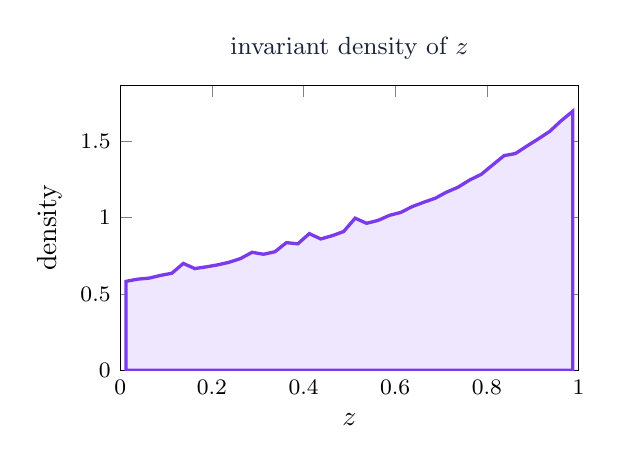
\begin{tikzpicture}
\begin{axis}[width=7.4cm,height=5.2cm,title={\small invariant density of $z$},xlabel={$z$},ylabel={density},xmin=0,xmax=1,ymin=0,tick label style={font=\footnotesize},title style={color=ink}]
\addplot[acc,very thick,fill=acc!12] coordinates{(0.0125,0.583) (0.0375,0.5973) (0.0625,0.604) (0.0875,0.6219) (0.1125,0.6362) (0.1375,0.7005) (0.1625,0.6668) (0.1875,0.678) (0.2125,0.6911) (0.2375,0.7081) (0.2625,0.7327) (0.2875,0.7734) (0.3125,0.7605) (0.3375,0.7771) (0.3625,0.8366) (0.3875,0.829) (0.4125,0.8958) (0.4375,0.8608) (0.4625,0.8822) (0.4875,0.9096) (0.5125,0.997) (0.5375,0.9634) (0.5625,0.9824) (0.5875,1.0155) (0.6125,1.0351) (0.6375,1.0735) (0.6625,1.1016) (0.6875,1.128) (0.7125,1.1683) (0.7375,1.2006) (0.7625,1.2472) (0.7875,1.2836) (0.8125,1.3454) (0.8375,1.4066) (0.8625,1.4208) (0.8875,1.4697) (0.9125,1.517) (0.9375,1.5664) (0.9625,1.6363) (0.9875,1.6972)} \closedcycle;
\end{axis}\end{tikzpicture}\hfill
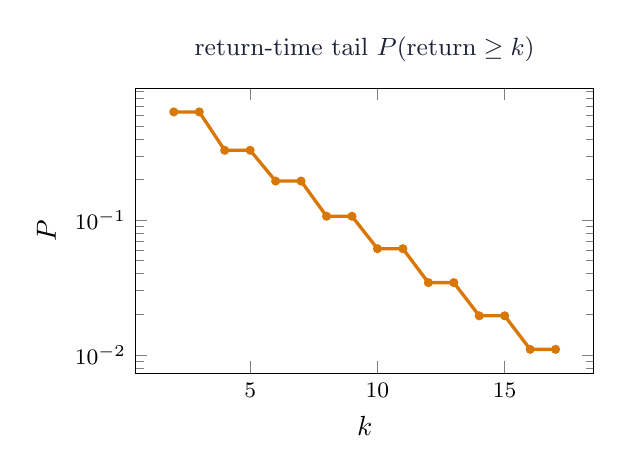
\begin{tikzpicture}
\begin{semilogyaxis}[width=7.4cm,height=5.2cm,title={\small return-time tail $P(\text{return}\geq k)$},xlabel={$k$},ylabel={$P$},tick label style={font=\footnotesize},title style={color=ink}]
\addplot[warm,very thick,mark=*,mark size=1pt] coordinates{(2,0.63525) (3,0.63525) (4,0.32979) (5,0.32979) (6,0.19493) (7,0.19493) (8,0.10685) (9,0.10685) (10,0.06137) (11,0.06137) (12,0.03437) (13,0.03437) (14,0.01949) (15,0.01949) (16,0.01098) (17,0.01098)};
\end{semilogyaxis}\end{tikzpicture}
\end{center}
\noindent Density is smooth, monotone, BV-looking; the tail is log-linear (slope $-0.284$)---\emph{geometric}, i.e.\ summable, exactly as ``no long neutral runs'' predicts. Each branch is a M\"obius map in $z$ (an affine map on $(a,b)$ projectivized), so bounded distortion is classical.

\section{The Rychlik reduction: what remains}
\begin{theorem}[Conditional almost-all, via Rychlik]
If the induced $F$-return map satisfies \emph{(i)} $\inf_z|g'(z)|=\lambda>1$ and \emph{(ii)} $\sum_{\text{branches}}\mathrm{var}(1/|g'|)<\infty$, its transfer operator is quasi-compact on $BV$: a unique a.c.\ invariant measure with exponential mixing. With the positive drift $E_\mu[\log|F'|]=0.134>0$ and Borel--Cantelli on the summable fatal hazard, \textbf{almost all seeds never die.}
\end{theorem}
\textbf{Now rigorous:} the no-intermittency grammar; the M\"obius/bounded-distortion branch structure; qualitative uniform expansion and geometric tails. \textbf{Remaining} (bounded, checkable---not open-ended): a rigorous $\lambda>1$ bound (numerics say $\lambda\!\approx\!4$, large margin) and a rigorous $\sum\mathrm{var}(1/|g'|)<\infty$ bound (from M\"obius distortion $+$ the $-0.284$ tail). Two constants for an explicit finite-data map. \emph{No theorem is claimed until these close.}

\section{Other ways through the door}
\begin{center}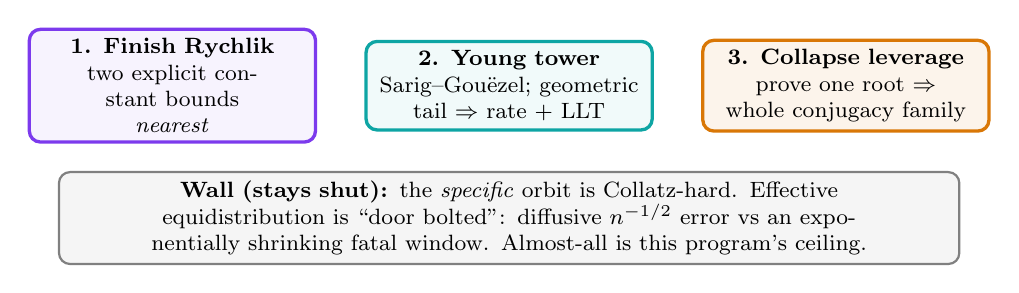
\begin{tikzpicture}[>=Latex,font=\footnotesize,node distance=6mm]
\node[draw=acc,very thick,rounded corners,fill=acc!6,text width=3.4cm,align=center](r1){\textbf{1. Finish Rychlik}\\two explicit constant bounds\\\textit{nearest}};
\node[draw=acc2,very thick,rounded corners,fill=acc2!6,text width=3.4cm,align=center,right=of r1](r2){\textbf{2. Young tower}\\Sarig--Gou\"ezel; geometric tail $\Rightarrow$ rate + LLT};
\node[draw=warm,very thick,rounded corners,fill=warm!8,text width=3.4cm,align=center,right=of r2](r3){\textbf{3. Collapse leverage}\\prove one root $\Rightarrow$ whole conjugacy family};
\node[draw=gray,thick,rounded corners,fill=gray!8,text width=11.2cm,align=center,below=5mm of r2](wall){\textbf{Wall (stays shut):} the \emph{specific} orbit is Collatz-hard. Effective equidistribution is ``door bolted'': diffusive $n^{-1/2}$ error vs an exponentially shrinking fatal window. Almost-all is this program's ceiling.};
\end{tikzpicture}\end{center}

\noindent\textbf{Honesty.} Every number is a measurement; the parity grammar is a proof. Tao \emph{proved} his theorem; we have proven the enabling structural fact and reduced ours to two standard constants with strong numerics---closer to the door, not through it. Nothing here bears on any specific machine's unconditional non-halting.
\end{document}